\begin{aufgabe}
	Das Blech hat eine Stärke von \SI{1}{cm} und eine Dichte von \SI{2700}{kg/m^3}.
	Zeichnen Sie die Gewichtskraft ein. Zerlegen Sie die Gewichtskraft grafisch in eine Komponente parallel zum Hebelarm (Sp--D),
	und eine senkrecht zum Hebelarm.
	Berechnen Sie die Grösse des Drehmoments?

	\begin{center}
		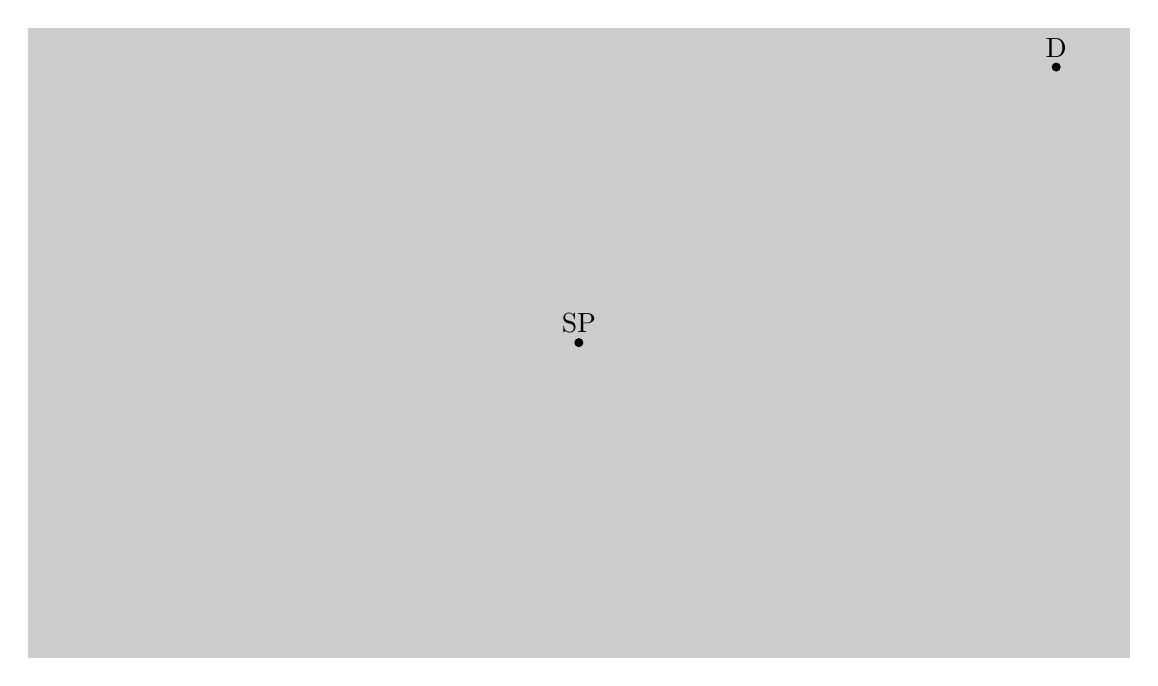
\begin{tikzpicture}
		\fill [color=black!20] (-7,4) rectangle (7,-4);
		\draw [fill] (0,0) circle (0.05) node [above] {SP};
		\draw [fill] (0,0) (30:7) circle (0.05) node [above] {D};	
		\end{tikzpicture}
	\end{center}

\end{aufgabe}


